\numberedsection{RF5.4 Borrar relación}

\subsection*{Descripción}
Permite a los usuarios eliminar una relación existente en el sistema.\par
\vspace{0.15cm}

\textbf{Pre-condición}\par
El usuario debe tener la sesión iniciada en Mini PIM. La relación a eliminar debe de existir en el sistema.\par
\vspace{0.15cm}

\textbf{Post-condición}
\begin{itemize}
    \item Caso de éxito: La relación es eliminada correctamente, se elimina de la lista de relaciones y se actualiza la base de datos.
    \item Caso mínimo: El sistema notifica al usuario el resultado de la acción de borrar relación: exitosa o fallida.
\end{itemize}

\textbf{Prioridad: }
Alta
\vspace{0.15cm}

\textbf{Autor: }
Pablo Ortega Serapio\par
\vspace{0.15cm}

\textbf{Control de cambios: } Versión 1: Definición del caso de uso

\numberedsubsection{Escenario principal}
\begin{enumerate}
    \item El usuario ha iniciado sesión con su cuenta de usuario correspondiente.
    \item El usuario accede a la sección de gestión de relaciones.
    \item El sistema muestra la lista de relaciones existentes.
    \item El usuario selecciona la opción de \enquote{Eliminar} una relación.
    \item El sistema muestra una ventana emergente de confirmación para la eliminación de la relación.
    \item El usuario confirma la eliminación.
    \item El sistema elimina la relación de la base de datos.
    \item El sistema actualiza la lista de relaciones, eliminando la relación seleccionada.
    \item El sistema muestra la lista de relaciones actualizadas.
\end{enumerate}

\numberedsubsection{Escenarios alternativos}
\begin{description}
  
    \item[4.a] El usuario cancela la acción de eliminar la relación seleccionada.
    \begin{enumerate}
        \item[4.a.1] El sistema regresa a la sección de gestión de relaciones sin realizar ningún cambio.
    \end{enumerate}
\end{description}

\numberedsubsection{Casos de Prueba}
\underline{Escenario: Principal}\par
\vspace{0.15cm}

\textbf{Dado} que he iniciado sesión con mi cuenta de usuario correspondiente,\par
\textbf{Y} estoy en el apartado de relaciones,\par
\textbf{Cuando} selecciono la opción de \enquote{Eliminar} en una relación,\par
\textbf{Y} confirmo la eliminación de la relación en la ventana emergente,\par
\textbf{Entonces} el sistema elimina la relación de la base de datos,\par
\textbf{Y} actualiza la lista de relaciones, removiendo la relación eliminada,\par
\textbf{Y} muestra la lista de relaciones actualizadas.\par

\vspace{0.20cm}

\underline{Escenario: Alternativo 4.a}\par
\vspace{0.15cm}

\textbf{Dado} que he iniciado sesión con mi cuenta de usuario correspondiente,
\textbf{Y} estoy en el apartado de relaciones,\par
\textbf{Cuando} selecciono la opción de \enquote{Eliminar} en una relación,\par
\textbf{Y} selecciono la opción de \enquote{Cancelar} en la ventana emergente,\par
\textbf{Entonces} el sistema regresa a la sección de gestión de relaciones,\par
\textbf{Y} muestra la lista de relaciones sin realizar ningún cambio.\par


\vspace{0.20cm}

\numberedsubsection{Bocetos}
\begin{figure}[H]
    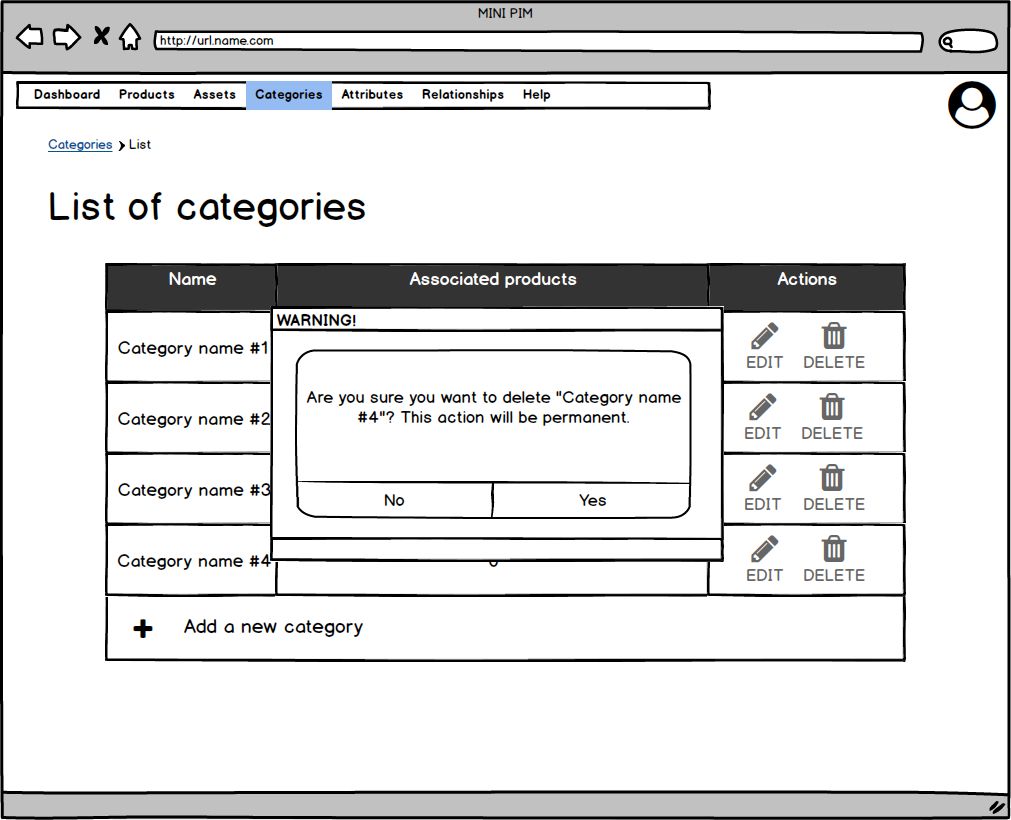
\includegraphics[width=1\linewidth]{mockups/RF4.4_1.png}
    \caption{Mensaje esperando confirmación para eliminar relación}
   \end{figure}
\vspace{1.0cm}

\begin{figure}[H]
    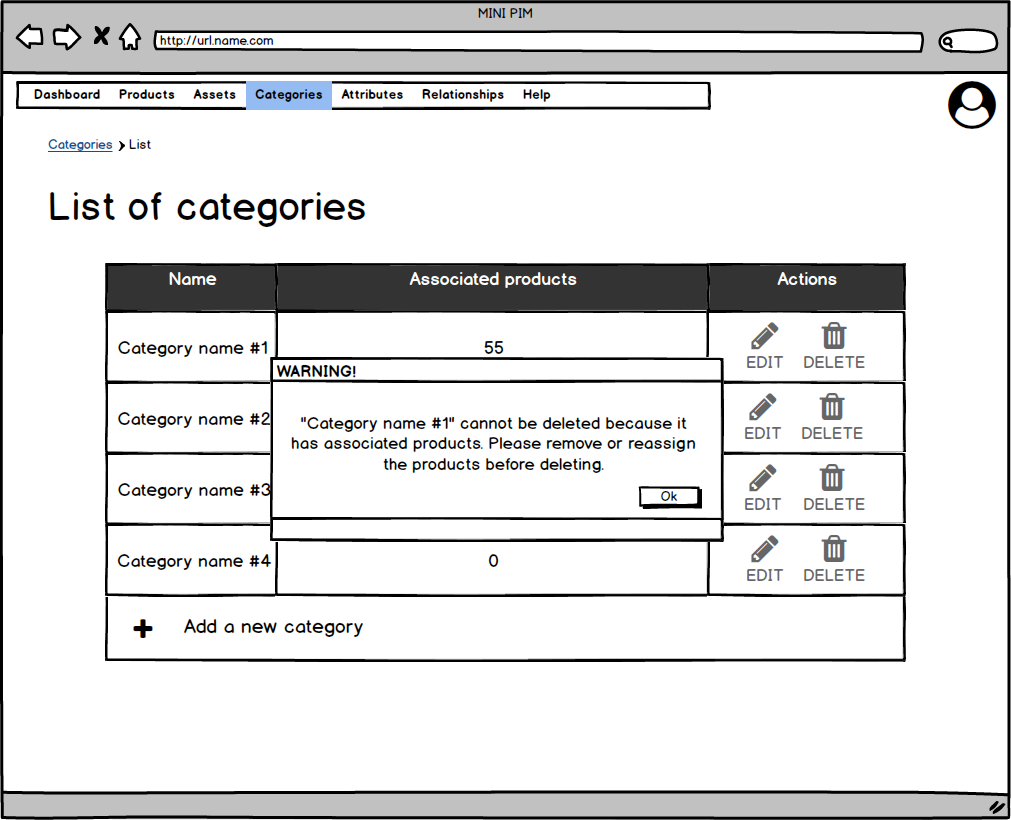
\includegraphics[width=1\linewidth]{mockups/RF4.4_2.png}
    \caption{Mensaje de error porque la relación a borrar tiene productos asociados}
   \end{figure}
\vspace{1.0cm}

\newpage %Inicia en una nueva página otro caso de uso